\chapter{狭义相对论}
\section{相对性原理}
\paragraph{参考系}
为了描述自然界中发生的过程,我们必须要有一个参考系,它包含了一个坐标系和一个固定在参考系中的钟.
\paragraph{惯性系}
如果一个不受外界作用的物体,在参考系中静止或者做匀速直线运动,这样的参考系称为惯性系.狭义相对论中涉及的参考系全部都是惯性系.如果存在一
个基本惯性系，相对于此惯性系做匀速直线运动的另一坐标系也是一个惯性系。
\paragraph{}{\kaishu 这不是显然的,因为它涉及到了速度的参考系变换:如果在K系中存在速度为常数u的物体和速度为常数v的参考系K',那么在K'系中物体的速度u'也是一个常数(所以K'是惯性系).然而在确定K'是惯性系之前,我们不能应用任何关于惯性系的原理和物理定律.因此最后一句话不是一个推论,而是一个同样重要的假设或者定义:牛顿第一定律成立的参考系是一个基本惯性系,相对于惯性系静止或者匀速运动的参考系称为惯性系.事实上后半句才是惯性系的定义,牛顿第一定律(关于惯性系性质的公设)的引入帮助我们确定了最初的基本惯性系."不受外界作用"可以理解为孤立的、远离其它粒子的,从而避免了依赖牛顿第一定律进行判断引发"先有鸡还是先有蛋"的问题.}
\paragraph{狭义相对论基本假设}
\begin{itemize}
    \item \tbf{相对性原理}:所有的自然定律在所有惯性系中是相同的.
    \item \tbf{光速不变原理}:物体之间的相互作用不是瞬时的,从一个物体向另一个物体发出的相互作用称做"信号",信号传播速度(光速)在不同惯性系中是相同的(相对性原理).\[ c=2.998\times 10^8 m/s\]
\end{itemize}
\subsection{经典力学的时空观}经典力学中的空间观念是相对的,当我们说不同时刻的两个事件发生在同一地点时,必须指明参考系才有意义.比如火车上一只苍蝇飞起,盘旋一会儿后落回了原来的位置,就是相对火车上的乘客而言的,但是对大地参考系却不是这样.经典力学的时间观念是绝对的,纯粹均匀地流逝而不因参考系的选择而变化.
\subsection{相对论的时空观}
\paragraph{同时的相对性}
考虑一个匀速行驶的长度为2L的车厢,车厢顶部挂有一个灯泡.现在打开灯泡,在车厢参考系中光线以相同的速度c向车厢两边传播,同时到达车厢的(a)(b)两端.但是在地面参考系中,光线从灯泡初始时刻的位置发出后,以相同的速度c(而不是c-v和c+v)向车厢两端传播,与此同时车厢在向右运动,光线相对于车厢左端(b)的速度是c+v,而相对于(a)的速度是c-v,因此光线将先到达(b)端.注意,光速不变是相对于参考系的,而不是参考系中被描述的其它物体的.
\paragraph{钟慢效应}
\paragraph{尺缩效应}
\begin{figure}
    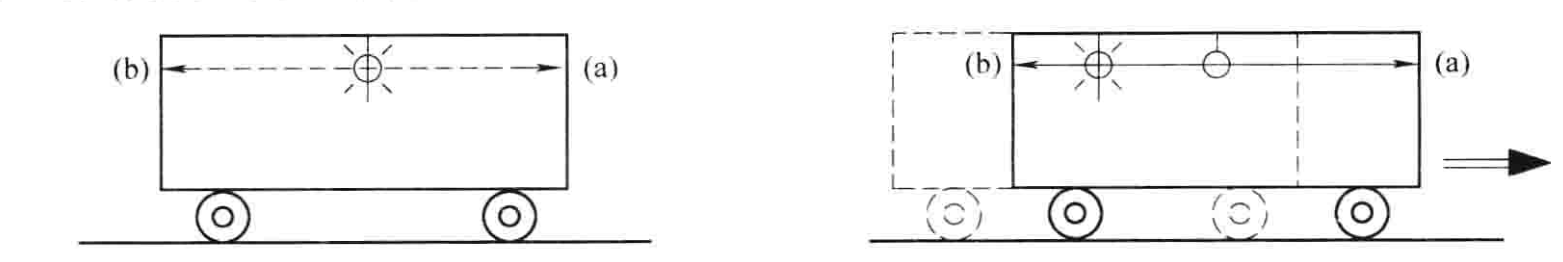
\includegraphics[width=\linewidth]{figure/relativity/1.png}
    \caption{同时的相对性}
\end{figure}
\section{间隔}
\paragraph{事件}指的是时间和空间中的一个点，在四维坐标系下用世界点(t, x, y, z) 来刻画。所有事件的集合构成了我们的时空。然而，需要强调的是事件本身与坐标系选择无关，在不同坐标系下事件的坐标是不同的。而世界线（worldline）指的是一个点粒子在时空中的轨迹。
$s_{12}$称为间隔,不同参考系中的间隔是相等的(这样的量称为洛伦兹不变量,LI),利用间隔的这种性质可以方便地求出不同惯性系中坐标和时间的变换关系.我们采用高能物理常用的西海岸约定(+---),而在天体物理中常用东海岸约定(-+++).
\begin{equation}
    s_{12}^2=(c(t_2-t_1))^2-(x_2-x_1)^2-(y_2-y_1)^2-(z_2-z_1)^2=c^2t_{12}^2-l_{12}^2
\end{equation}
$s_{12}$是虚数,即$s_{12}^2>0$的间隔称为\tbf{类时间隔},类时间隔两端的事件可以在某个参考系中同一点发生:
\begin{equation}
    s_{12}^2=c^2 t_{12}^2-l_{12}^2=c^2 {t'}_{12}^{2} \qquad {l'}_{12}^{2}=0
\end{equation}
类似的还有\tbf{类空间隔},$s_{12}^2<0$,如果两个事件的间隔是类空间隔,那么他们可能在某个参考系中同时发生:
\[s_{12}^2=c^2 t_{12}^2-l_{12}^2=-c^2 {l'}_{12}^{2} \qquad {t'}_{12}^{2}=0\]
还有\tbf{类光间隔},如果$s_{12}^2=0$,这与光的传播类似.

\section{洛伦兹变换}
\paragraph{洛伦兹变换} 从一个惯性系中坐标(x,y,z,t)到另一个惯性系中(x',y',z',t')的变换公式称为洛伦兹变换.如果我们在有三个空间实轴x,y,z和一个虚轴ict四维闵可夫斯基空间考虑参考系变换的问题,不难发现,间隔对应两个世界点在四维坐标系中的距离.参考系变换就是将世界点的在一套坐标系中的坐标变换到另外一套坐标轴中对应的坐标,保持"距离"不变的坐标的变换只有两种:旋转和平移.而平移只涉及空间坐标原点和零时刻的选择,所以我们所要求的变换对应坐标轴的转动.
\paragraph{}假设K'系相对K系沿x方向以速度v运动:
\begin{equation}
    \begin{pmatrix}
        \cosh\psi&\sinh\psi\\
        \sinh\psi&\cosh\psi
    \end{pmatrix}
    \begin{pmatrix}
        x'\\t'
    \end{pmatrix}
    =\begin{pmatrix}
        x\\t
    \end{pmatrix}
\end{equation}
在伪欧几里得几何的转动矩阵中三角函数被双曲函数取代.考虑K'系的原点x'=0在K系中的坐标x:
\begin{equation}
    x=ct'\sinh\psi\qquad ct=ct'\cosh\psi 
\end{equation}
于是我们得到
\begin{equation}
    \tanh\psi=\frac{x}{ct}=\frac{v}{c}
\end{equation}
由此得到了从运动系K'到静止系K的变换公式,亦即著名的\tbf{洛伦兹变换}:
\begin{equation}
        x=\gamma(x'+vt')\quad t=\gamma(t'+\frac{v}{c^2}x') \quad y=y' \quad z=z'
\end{equation}
其中$\gamma=\frac{1}{\sqrt{1-\frac{v^2}{c^2}}},\beta=\frac{v}{c}$.反之:
\begin{equation}
    x'=\gamma(x-vt)\quad t'=\gamma(t-\frac{v}{c^2}x) \quad y'=y \quad z'=z
\end{equation}
我们还可以得到速度$\mathbf{u}=\dv{\mathbf{r}}{t}$的变换公式:
\begin{equation}
    \begin{aligned}
        &\dd{x}=\gamma(\dd x'+v\dd{t}')\quad \dd t=\gamma(\dd t'+\frac{v}{c^2}\dd x') \quad \dd y=\dd y' \quad \dd z=\dd z'\\
        &u_x=\frac{u'_x}{\sqrt{1+u'_xfrac{v}{c^2}}}\quad u_y=\frac{1/\gamma u'_y}{\sqrt{1+u'_xfrac{v}{c^2}}}
        \quad u_z=\frac{1/\gamma u'_z}{\sqrt{1+u'_xfrac{v}{c^2}}}
    \end{aligned}
\end{equation}
\section{四维矢量}
用以下方法表示洛伦兹变换时,形式会简化许多:
\begin{equation}
    \begin{gathered}
        x^{\mu}=\{ct,x,y,z\}\quad x_{\mu}=\{ct,-x,-y,-z\}\\
    \end{gathered}
\end{equation}
\begin{equation}
    \begin{pmatrix}
        {x'}^{0}\\{x'}^1\\{x'}^2\\{x'}^3
    \end{pmatrix}
    =\begin{pmatrix}
        \gamma&-\beta\gamma&0&0\\
        -\beta\gamma&\gamma&0&0\\
        0&0&1&0\\
        0&0&0&1
    \end{pmatrix}
    \begin{pmatrix}
        x^0\\x^1\\x^2\\x^3
    \end{pmatrix}
\end{equation}
或者用张量的形式写为:
\begin{equation}
    {x'}^{\mu}=\sum_{\nu=0}^{3}\Lambda_{\nu}^{\mu}x^{\nu}=\Lambda_{\nu}^{\mu}x^{\nu}
\end{equation}
我们引入\tbf{爱因斯坦求和规则}:当出现重复指标时就意味着求和,而把求和号省略掉.每对指标中必须一个上标,另一个为下标.这种"傀"指标用起来非常方便.
\paragraph{四维矢量}
在洛伦兹变换下与$x^{\mu}$有相同变换规则的一组四分量矢量称为4-矢量:
\begin{equation}
    {a'}^{\mu}=\Lambda_{\nu}^{\mu}a^{\nu}
\end{equation}
$a^{\mu}$称为逆变矢量,$a_{mu}$称为协变矢量.
\begin{gather}
    a^{\mu}=(a^0,a^1,a^2,a^3)=g^{\mu\nu}a_{\nu}\\
    a_{\mu}=(a^0,-a^1,-a^2,-a^3)=g_{\mu\nu}a^{\nu}\\
    g_{\mu\nu}=g^{\mu\nu}=\begin{pmatrix}
        1&0&0&0\\
        0&-1&0&0\\
        0&0&-1&0\\
        0&0&0&-1
    \end{pmatrix}
\end{gather}
在引入了四维矢量之后,间隔也可以改写为:
\begin{equation}
    s=x^{\mu}x_{\mu}
\end{equation}
它是一个\tbf{四维标量积},正如普通的点积在三维坐标转动下是不变的,四维标量积在洛伦兹变换下也是不变的,称为\tbf{洛伦兹不变量(Lorentz Invariant,LI)}